% !TeX root=../main.tex
\chapter{مروری بر مطالعات انجام شده}
%\thispagestyle{empty} 
\section{مقدمه}
در مقاله\cite{Nakamoto2009}، در کنار معرفی بیت‌کوین، روشی به نام درستی سنجی پرداخت ساده‌شده (SPV) معرفی شده است. در این روش، امکانی به شبکه بیت‌کوین اضافه گشت که دسته‌ای از کاربران، بدون نیاز به راه‌اندازی یک گره کامل، بتوانند با اثبات مرکلی که از یک گره کامل دریافت می‌کنند، تایید کنند که یک تراکنش درون زنجیره بلوکی بیت‌کوین ثبت گردیده‌ است یا خیر. به این کاربران، کاربر سبک و به گره آن‌ها در شبکه بیت‌کوین، گره سبک گفته می‌شود. گره‌های سبک یا به عبارت دیگر گره‌هایی که در وضعیت تایید ساده‌شده پرداخت‌ها عمل می‌کنند، نیازی به ذخیره تمام زنجیره بلوکی وجود ندارد. این گره‌ها تنها سرایند زنجیره بلوکی را از شبکه دریافت و ذخیره می‌کنند.  هرچند که در این روش کاربران سبک نیاز به بارگیری تمام زنجیره بلوکی بیت‌ کوین را ندارند و تنها لازم است که سرایند بلوک‌ها را ذخیره کنند،‌ اما عملکرد صحیح آن‌ها در گرو ارتباط آن‌ها با یک گره کامل درست کار است. اگرچه گره‌های سبک می‌توانند تایید کنند که سرایند بلوک‌هایی که دریافت کرده‌اند اثبات کار صحیحی دارند یا خیر اما بدون داشتن تمام زنجیره بلوکی نمی‌توانند مطمئن شوند که تمام تراکنش‌های موجود در بلوک‌ها کاملا درست هستند.

آسیب‌پذیری دیگری که گره‌های سبک را تهدید می‌کند، عدم حفظ حریم خصوصی آن‌ها در مقابل گره‌های کاملی است که از آن‌ها درخواست اطلاعات می‌نمایند. یکی از اصلی‌ترین اطلاعاتی که گره‌های سبک از گره‌های کامل درخواست می‌کنند تراکنش‌های مربوط به آدرس(های) گره سبک است. کاربر سبک علاوه بر تراکنش مورد نظر، چکیده بلوکی که تراکنش در آن قرار دارد و همچنین اثبات مرکل وجود آن تراکنش در آن بلوک را دریافت می‌کند. در صورتی که گره سبک به صورت فاش اطلاعات آدرس خود را در اختیار گره کامل قرار دهد، گره کامل خواهد توانست اولا، ارتباط آدرس‌های بیت‌کوین گره سبک با آدرس آی‌پی وی را کشف نماید و در نهایت بفهمد که دارنده این آدرس در کدام موقعیت جغرافیایی قرار دارد (اگر کاربر سبک از شبکه‌های حافظ گم‌نامی استفاده نماید این امکان برای گره کامل وجود نخواهد داشت). ثانیا، این امکان به گره کامل داده می‌شود که بتواند از این طریق ارتباط بین آدرس‌های یک شخص را در شبکه بیت‌کوین ساده‌تر کشف کند. کشف آن که کدام آدرس‌های بیت‌کوین مربوط به یک کاربر به خصوص است، می‌تواند به کشف الگوی رفتاری آن کاربر و در نتیجه کشف نسبی هویت آن منجر شود \cite{Ron2013}. از این رو فاش شدن هر دوی این اطلاعات حریم خصوصی کاربر سبک را نقض خواهد کرد.

به این ترتیب،‌ گره سبک به خاطر اعتماد به یک یا چند گره کامل و نقض حریم خصوصیش از امنیت کمتری نسبت به گره‌های کامل برخوردار است \cite{Sompolinsky2016}. از این رو تاکید می‌شود کاربرانی که مقدار زیادی بیت‌کوین را نگهداری یا مبادله می‌کنند، یا کاربرانی که می‌خواهند گم‌نامی آن‌ها حفظ شود از گره‌ کامل استفاده کنند. با این حال لازم است که تلاش شود امنیت، به ویژه گم‌نامی، کاربران سبک تا حد امکان تامین گردد. چرا که فاش شدن اطلاعات بخشی از اعضای شبکه می‌تواند منجر به فاش شدن اطلاعات دیگر بخش‌های شبکه گردد.

برای حل مشکل فاش شدن آدرس مربوط به گره سبک نزد گره کامل متخاصم، در پروتکل فعلی بیت‌کوین از فیلتر بلوم استفاده می‌شود \cite{Hearn2013}. در مقاله \cite{Gervais2014} توضیح داده ‌شد که استفاده از فیلتر بلوم از امنیت کافی برخوردار نیست. در این فصل پایان‌نامه به معرفی فیلتر بلوم، نحوه استفاده آن در شبکه همتا‌به‌همتای بیت‌کوین و ضعف‌های آن به عنوان ابزاری جهت حفظ حریم خصوصی کاربران خواهیم پرداخت.

\section{تعاریف، اصول و مبانی نظری}
فیلتر بلوم هم اکنون در کیف پول‌هایی نظیر بیت‌کوین‌جِی\RTLfootnote{\lr{Bitcoinj}} \cite{bitcoinj} استفاده می‌شود. در این بخش به معرفی این فیلتر و همچنین نحوه به کارگیری آن در شبکه همتا-به‌همتای بیت‌کوین و آسیب‌پذیری‌های آن پرداخته شده است.

\subsection{تراکنش‌ در بیت‌کوین}

\subsection{فیلتر بلوم}
فیلتر بلوم را نخستین بار برتون بلوم در \cite{Bloom1970} معرفی کرد. هدف این فیلتر امتحان سریع وجود یک عضو در یک مجموعه است. فیلتر بلوم کاربرد گسترده‌ای در پایگاه‌های داده، شبکه و حتی موتور‌های جست‌وجو دارد. فیلتر بلوم آرایه‌ای از $n$ بیت $b[i]$ است که $i$ از $0$ تا$n-1$ است. به صورت پیش‌فرض تمام بیت‌ها مقدار صفر دارند. اگر بخواهیم عضو $x$ را (مثلا یک رشته) درون مجموعه آن قرار دهیم، آن عضو را در ورودی $k$ تابع چکیده‌ساز مستقل
$H_1(.), H_2(.), ..., H_k(.)$
قرار می‌دهیم. خروجی هر تابع چکیده ساز یک عدد صحیح بین $0$ تا $n-1$ است. از این رو هر تابع چکیده ساز، یک عنصر ورودی را به یکی از	 $n$ بیت فیلتر بلوم نگاشت می‌کند. برای قرار دادن آن رشته در مجموعه مربوط به فیلتر بلوم، بیت متناظر عدد حاصل را برابر با یک قرار می‌دهیم: 

$\forall j\in \{1..k\}, b[H_j(x)] \leftarrow 1$.

به همین ترتیب اگر بخواهیم بررسی کنیم که یک رشته در مجموعه قرار دارد، چکیده آن رشته را توسط همان $k$ تابع چکیده‌ساز حساب نموده و بررسی می‌کنیم که آیا مقدار ذخیره شده در تمام $k$ جایگاه بدست آمده برابر یک است یا خیر. اگر برابر با یک باشد، آن رشته را عضو احتمالی آن مجموعه در نظر می‌گیریم. به آن عضو احتمالی گفته می‌شود چرا که ممکن است عناصری عضو مجموعه نباشند و به جایگاه‌هایی که مقدار  بیت آن‌ها برابر با یک است نگاشت شوند. به این ترتیب امکان بروز خطای نوع دو وجود دارد. مجموعهٔ تمامی عناصر با $\mathcal{U}$، اعضایی که درون فیلتر بلوم قرار گرفته‌اند با $\mathcal{S}$ و مجموعهٔ عناصری که در نتیجه خطای نوع دو عضو فیلتر بلوم در نظر گرفته می‌شوند با $\mathcal{V}$ نمایش داده می‌شوند. به صورت کلی می‌توان گفت هرگاه لیست یا مجموعه‌ای مورد استفاده قرار گرفت، هزینه فضای ذخیره‌سازی و دسترسی به اعضای مجموعه قابل توجه بود و خطای نوع دو خسارت و هزینه چندانی به سامانه تحمیل نکند، استفاده از فیلتر بلوم مفید خواهد بود. فیلتر بلوم امکان انجام مصالحه بین فضای استفاده شده، زمان پاسخ‌گویی و احتمال خطای قابل قبول را فراهم می‌کند\cite{Bloom1970}. با توجه به ساختار فیلتر بلوم روشن است که امکان بروز خطای نوع یک، یا به عبارت دیگر امکان آنکه عضو مجموعه را غیر عضو تشخیص دهد، وجود ندارد.

\begin{figure}
	\centering
	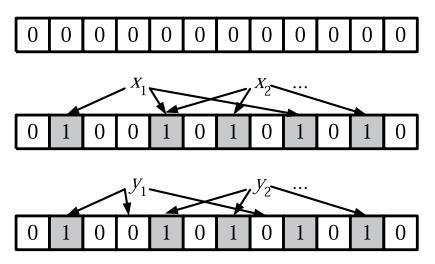
\includegraphics[width=0.55\linewidth]{image/BloomFilter}
	\caption[نمونه‌ای از عمکلرد فیلتر بلوم]{
		فیلتر مجموعه بدون عضو متشکل از یک آرایه‌ از بیت‌ها با مقدار صفر است. k دفعه چکیده هر عضو مجموعه $x_i$ محاسبه می‌شود که حاصل هر چکیده موقعیت یک بیت است. که مقدار این بیت‌ها ۱ می‌شود. حال برای آنکه بررسی کنیم که $y_i$ درون این مجموعه است به تعداد k بار از آن چکیده می‌گیریم و بیت‌های مرتبط را بررسی می‌کنیم. عنصر $y_1$ نمی‌تواند عضو مجموعه باشد چرا که یکی از بیت‌هایی که به آن اشاره می‌کند صفر است. عنصر $y_2$ یا عضو مجموعه است یا اینکه به خاطر خطای نوع دو فیلتر، عضو مجموعه تشخیص داده شده است.\cite{Broder2004}
	}
	\label{fig:bloomfilter}
\end{figure}

در فیلتر بلوم برای تنظیم نرخ قابل قبول خطای نوع دوم ($P_t$)، با توجه به حداکثر تعداد عناصری که در فیلتر قرار خواهند گرفت($M$)، اندازه فیلتر($n$) و تعداد توابع‌ چکیده‌ساز($k$) تعیین می‌شوند.
جدول \ref{table:BloomFilter} نشانه‌گذاری‌های مربوط به فیلتر بلوم را نشان می‌دهد.

\begin{table}[h]
	\centering
	\caption{قرارداد نشانه‌گذاری برای فیلتر بلوم}
	\label{table:BloomFilter}
	\begin{tabular}{|c|c|}
		\hline
		نشانه‌گذاری & معنا \\
		\hline
		\hline
		$\mathcal{S}$ & مجموعه عناصری که عضو فیلتر شده‌اند \\
		\hline
		$M$ & حداکثر تعداد عناصر فیلتر\\
		\hline
		$m = |\mathcal{S}|$ & تعداد عناصر قرار داده شده در فیلتر\\
		\hline
		$n$ & اندازه (تعداد بیت‌های) فیلتر \\
		\hline
		$k$ & تعداد توابع چکیده‌ساز\\
		\hline
		$\mathcal{U}$ & مجموعهٔ تمام عناصر، $|\mathcal{U}| = N_u$ \\
		\hline
		$\mathcal{V}$ & مجموعهٔ پنهان‌سازی (عناصر خطای نوع دو)، $|\mathcal{V}| = N_v$\\
		\hline
		$P_t$ & نرخ (احتمال) خطای نوع دوی هدف (ایده‌آل)\\
		\hline
		$P_f$ & نرخ (احتمال) خطای نوع دوی واقعی \\
		\hline
		$B(M, P_t)$ & فیلتر بلوم با حداکثر ظرفیت $M$ و نرخ خطای نوع دو هدف $P_t$ \\
		\hline
	\end{tabular}
\end{table}

برای فیلتر بلوم
$B(M, P_t)$
اندازه فیلتر به صورت زیر محاسبه می‌شود\cite{Gervais2014}:

\begin{equation}
n=-\frac{M\ln(P_t)}{\left(\ln(2)\right)^2} \label{eq:n_of_bloom_filter}
\end{equation}
و تعداد توابع چکیده‌ساز به صورت زیر محاسبه می‌گردد\cite{Gervais2014}:
\begin{equation}
k=\ln(2)\frac{n}{M} \label{eq:k_of_bloom_filter}
\end{equation}
احتمال خطای نوع دو فیلتر بلوم
$B(M, P_t)$
، در صورتی که $m$ عنصر در آن قرار دهیم 
$(m<M)$

با دقت‌های متفاوتی محاسبه شده است. مقاله \cite{Bloom1970}، که فیلتر بلوم را معرفی کرده است، احتمال خطای نوع دو را برای فیلتر بلوم محاسبه کرده است. این مقاله با فرض این‌که بعد از قرار دادن $m$ عضو در فیلتر بلوم نسبت بیت‌هایی مقدار آن‌ها صفر مانده است به کل بیت‌ها برابر
$(1-k/n)^m$
باشد، احتمال خطای نوع دو را به صورت زیر محاسبه کرده است:

\begin{equation}
P_f(m) = \left(1-\left(1-\frac{k}{n}\right)^{m}\right)^k \label{eq:Pf_of_bloom_filter_Bloom}
\end{equation}

مقاله \cite{Mullin1983} محاسبه دقیق‌تری از احتمال خطای نوع دو به دست آمده است. در این مقاله، احتمال آن که یک بیت دلخواه بعد از مقدار دهی k بیت مقدارش عوض نشود،
$(1-1/n)^k$
محاسبه شده است. پس به این ترتیب بعد از قرار دادن $m$ عضو در فیلتر، احتمال آن‌که مقدار یک بیت تغییر نکند، برابر 
$(1-1/n)^{km}$
خواهد بود. در نتیجه احتمال آن‌که مقدار یک بیت تغییر کند به صورت 
$p_{set} = 1-(1-1/n)^{km}$
محاسبه می‌شود. پس احتمال خطای نوع دو برابر است با احتمال آن‌که تمام بیت‌های انتخابی حاصل از $k$تا چکیدهٔ عنصری که عضو فیلتر بلوم مورد نظر نیست،‌ از قبل مقدار یک گرفته باشند. به این ترتیب احتمال خطای نوع دو طبق اثبات \cite{Mullin1983}، به صورت زیر محاسبه می‌شود.

\begin{equation}
P_f(m) = \left(1-\left(1-\frac{1}{n}\right)^{km}\right)^k \approx \left(1-e^{-\frac{mk}{n}}\right)^k
\label{eq:Pf_of_bloom_filter_Mullin}
\end{equation}

برای $n\gg k$، مقادیر معادله‌های  \eqref{eq:Pf_of_bloom_filter_Mullin} و \eqref{eq:Pf_of_bloom_filter_Bloom} به هم نزدیک خواهند بود. مقاله \cite{Christensen2010} به فرمولی با دقت بیشتر از دو مقاله قبلی برای محاسبه احتمال خطای نوع دوی فیلتر بلوم دست پیدا کرده است که به شرح زیر است:

\begin{equation}
P_f(m) = \frac{n!}{n^{k(m+1)}} \sum_{i=1}^{n} \sum_{j=1}^{i} (-1)^{i-j} \frac{j^{km}i^k}{(n-i)!j!(i-j)!}
\label{eq:Pf_of_bloom_filter_Christensen}
\end{equation}


اثبات فرمول \eqref{eq:Pf_of_bloom_filter_Christensen} خارج از بحث این پایان‌نامه است. اگر تعداد پیام‌های قرارداده شده در فیلتر بلوم برابر با $M$ باشد، در آن صورت 
$P_f(M)=P_t$.


کاربرد‌های متعددی برای فیلتر بلوم وجود دارد و در ادامه یکی از آن‌ها را مرور خواهیم کرد. در وبسایت‌هایی که خدمات کوتاه‌کردن لینک را ارائه می‌کنند (مانند \cite{Bitly.comTeam2020})، معمولا لیست سیاهی از آدرس‌های غیر امن نگهداری می‌شود و به کاربر استفاده کننده از لینک‌های کوتاه‌شده اطمینان می‌دهد که آدرسی که به آن هدایت خواهد شد یک آدرس امن است (در لیست سیاه آدرس‌های ناامن قرار ندارد). جست‌وجو کردن لیست سیاه آدرس‌های ناامن برای هر درخواست امری زمان‌بر است. از این رو، مجموعهٔ تمام آدرس‌های ناامن در یک فیلتر بلوم نگهداری می‌شود. اگر پاسخ فیلتر بلوم برای یک آدرس درخواست داده شده منفی باشد (عضو مجموعه نباشد) می‌توانیم صددرصد مطمئن باشیم که آدرس در‌خواست داده شده یک آدرس امن است و اگر پاسخ مثبت باشد،‌ جهت جبران خطای نوع دو، پایگاه‌ داده لیست سیاه آدرس‌های ناامن را جست‌وجو می‌کند\cite{Azar2016}.

\textbf{\textit{\underline{یک کاربرد حریم خصوصی دیگر برای فیلتر بلوم}}}

کاربرد فیلتر بلوم مورد نظر در این پایان‌نامه، استفاده از آن در گره‌های سبک برای حفظ گم‌نامی این گره‌ها است \cite{Hearn2013}. در بخش‌  \ref{BloomFilterInP2P} به نحوه استفاده از این فیلتر در ارتباط بین گره‌های سبک و گره‌های کامل پرداخته می‌شود و در بخش \ref{Vulnerabilities} به ضعف‌ها و آسیب‌پذیری‌های استفاده از این فیلتر در شبکه بیت‌کوین خواهیم پرداخت. 


\subsubsection{فیلتر بلوم در شبکه همتا‌به‌همتای بیت‌کوین}
\label{BloomFilterInP2P}

امکان استفاده از فیلتر بلوم در ارتباط بین گره سبک و گره کامل در سال ۲۰۱۳ و به دنبال معرفی آن در طرح پیشنهادی بهبود بیت‌کوین شمارهٔ ۳۷ (\lr{BIP37}) \cite{Hearn2013} فراهم شد. همان‌طور که در بخش قبل گفته شد، گره‌‌های سبک برای حفظ گم‌نامی خود، به جای آن‌که آدرس‌های مربوط به خودشان را صورت فاش در اختیار یک گره کامل قراردهند، آدرس‌های خود را در یک فیلتر بلوم با نرخ خطای نوع دو معین قرار می‌دهند. پیاده‌سازی‌های نرم‌افزاری متعددی برای گره سبک یا به عبارت دیگر، کاربر SPV بیت‌کوین وجود دارد مانند بیت‌کوین‌جی \cite{bitcoinj}، الکترام \RTLfootnote{\lr{Electrum}} 
\cite{Electrum}
و پیکوکوین\RTLfootnote{\lr{PicoCoin}}
\cite{Garzik}. 
اصطلاحا، به نرم‌افزار‌های گره سبک، کیف پول\RTLfootnote{\lr{Wallet}} گفته می‌شود.

بیت‌کوین‌جی یک کتاب‌خانه کاربر سبک (SPV) به زبان جاوا \RTLfootnote{\lr{Java}} است. بیت‌کوین‌جی مستقیما با استفاده از پیام‌های استاندارد تعریف شده در شبکه همتا‌به‌همتای بیت‌کوین \cite{P2P_dev,P2P_ref} با گره کامل ارتباط برقرار می‌کند. این پیاده‌سازی از اکثر استاندارد‌های بیت‌کوین،‌از جمله فیلتر بلوم \cite{Hearn2013}  پشتیبانی می‌کند. در این پایان‌نامه به صورت کلی منظور از گره سبک یا کاربر \lr{SPV}، بیت‌کوین‌جی است. کاربر سبک بیت‌کوین‌جی به صورت همزمان می‌تواند به چند گره کامل متصل باشد و از طریق آن‌ها اطلاعاتش بروزرسانی گردد.


در پیاده‌سازی الکترام،‌ کاربر سبک مستقیما طبق پروتکل ارتباطی بیت‌کوین با گره کامل مبادلهٔ اطلاعات نمی‌کند. گره کاملی که زنجیره بلوکی بیت‌کوین را ذخیره کرده‌است،‌ لازم است برای ارائه خدمات به کاربران سبکی که از الکترام استفاده می‌کنند،‌ سرور 
الکترام‌ایکس\RTLfootnote{\lr{ElectrumX}}
\cite{ElectrumX}
  را در کنار نرم‌افزار گره کامل راه‌اندازی نمایند. در این پیاده‌سازی، برخلاف بیت‌کوین‌جی، گره سبک هم زمان به چند سرور الکتروم‌ایکس متصل نمی‌شود. بلکه به صورت تصادفی یک سرور را انتخاب می‌کند و به آن متصل می‌گردد. کاربر سبک خودش می‌تواند تعیین کند که به چه سروری متصل گردد. از این رو کاربر سبک می‌تواند  تنها اطلاعاتش را از گره کاملی که به آن اعتماد دارد به روز رسانی نماید.  همچنین در پروتکل ارتباطی گره سبک الکترام از فیلتر بلوم استفاده نمی‌شود. این ویژگی‌ها امنیت این پیاده‌سازی را با ابهام مواجه کرده است \cite{Alison2014}. 
  
  پیکوکوین،‌ یک کتاب‌خانه بیت‌کوین به زبان سی\RTLfootnote{\lr{C}} است. این کتاب‌خانه امکان استفاده به عنوان یک کیف‌پول بیت‌کوین و یک گره کامل را فراهم می‌کند. علاوه بر این، امکان ساخت نرم‌افزارهایی که مرتبط با بیت‌کوین هستند را ممکن می‌کند. این کیف پول از استاندارد ارتباطی بیت‌کوین تبعیت کرده و از فیلتر بلوم استفاده می‌کند، همچنین می‌تواند مستقیما به گره‌های کامل بیت‌کوین، بدون نیاز به راه‌اندازی سروری در سمت گره کامل، متصل شود.
  
  در این پژوهش هرگاه از گره سبک یا کاربر SPV صحبت می‌شود منظور کیف‌پول بیت‌کوین‌جی \cite{bitcoinj} و هر گاه از گره کامل صحبت می‌شود منظور پیاده‌سازی هسته بیت‌کوین \cite{Bitcoincore.org} هست. در ادامه به پروتکل ارتباط گره‌های سبک با گره‌های کامل و گرفتن اثبات مرکل  برای تراکنش‌های مورد نظر کاربر با بهره‌گیری از فیتلر بلوم پرداخته خواهد شد. 
  
\paragraph{یافتن همتا}

  اولین گامی که هر گره در شبکهٔ همتا‌به‌همتای بیت‌کوین انجام می‌دهد، یافتن گره‌های (همتا‌های) دیگر و اتصال به آن‌ها است. از آن‌جایی که آدرس آی‌پی گره‌های کامل فعال را در هنگام راه‌اندازی ندارد، از یک یا چند سرور 
 \RTLfootnote{\lr{Domain Name System}}\lr{DNS} 
 که آدرس‌ آن‌ها در کد بیت‌کوین‌جی از پیش قرارگرفته است پرسمان انجام می‌دهد. پاسخ دریافت شده شامل آدرس یک یا گره کاملی است که ارتباطات ورودی را قبول می‌کنند. علاوه بر این تعدادی آدرس گره کامل در کدهای بیت‌کوین‌جی قرار دارد که در زمانی که یک ورژن مشخص منتشر می‌شده فعال بوده‌اند. 
 \paragraph{اتصال به همتا}
 بعد از آن‌که کاربر جدید آدرس آی‌پی یک یا چند گره کامل را بدست آورد، برای آن کاربر(ان) پیام \texttt{Version} را ارسال می‌کند. این پیام برای ایجاد ارتباط ارسال می‌شود و شامل اطلاعاتی از گره ارسال کننده است. این اطلاعات در جدول  توضیح داده شده است.

 	
 \begin{xltabular}{\textwidth}{|c|X|}
 	\caption{
	قسمت‌های پیام \texttt{Version} در شبکه همتا‌به‌همتای بیت‌کوین
\label{table:VersionMessage}}\\
\hline
\textbf{نام} & {\centering
	\textbf{توضیحات}		
} \\
\hline
\hline
\lr{version} & {
	بالاترین نسخهٔ پروتکلی که توسط گره ارسال کننده شناخته می‌شود.	در زمان نگارش این پایان‌نامه، بالاترین نسخه پروتکل بیت‌کوین 70015 است که در سال ۲۰۱۷ منتشر شده است.
} \\
\hline
\lr{services} & {
	خدماتی که گره ارسال‌کننده پشتیبانی می‌کند را مشخص می‌کند. برای گره‌های سبکی مثل بیت‌کوین‌جی، مقدار آن برابر \texttt{0x00} است.
} \\
\hline
\lr{timestamp} & {
	ساعت یونیکس (\lr{Unix time}) با توجه به ساعت گره ارسال کننده در زمان ارسال پیام.
} \\
\hline
\lr{addr\_recv services} & {
	سرویس‌هایی که از دید گره ارسال‌کننده، توسط گره گیرنده پشتیبانی می‌شود. فرمت نمایش آن مانند قسمت services است. اگر گره ارسال‌کننده، بیت‌کوین‌جی باشد، همیشه به صورت پیش‌فرض مقدار این قسمت را برابر \texttt{0x00} قرار می‌دهد.
} \\
\hline
\lr{addr\_recv port} & {
	شماره پورت گره گیرنده از دید گره ارسال‌کننده.
}\\
\hline
\lr{addr\_trans services} & {
	خدماتی که گره ارسال‌کننده پشتیبانی می‌کند را مشخص می‌کند. یکسان با قسمت services باید باشد.
}\\

\hline
\lr{addr\_trans IP address} & {
	آدرس آی‌پی گره ارسال کننده.
}\\

\hline
\lr{addr\_trans port} & {
	شماره پورت گره ارسال کننده.
}\\

\hline
\lr{nonce} & {
	تک‌شمار، یک عدد تصادفی است که اگر یک گره،‌ یک پیام با تک‌شماری مشابه با تک‌شمار ارسالی دریافت کرد، ارتباط را قطع نماید. (قسمت تک‌شمار در ورژن $0.1.6$ بیت‌کوین اضافه شده و هدفش آن است که گره متوجه شود که به خودش متصل نشده است.)
	{\tiny  \lr{https://github.com/bitcoin/bitcoin/commit/cc0b4c3b62367a2aebe5fc1f4d0ed4b97e9c2ac9}}
}\\
\hline
\lr{user\_agent bytes} & {
	تعداد بایت‌هایی که قسمت \lr{user\_agent} (قسمت بعدی) استفاده کرده است.
}\\

\hline
\lr{user\_agent bytes} & {
	تعداد بایت‌هایی که قسمت \lr{user\_agent} (قسمت بعدی) استفاده کرده است.
}\\

\hline
 \end{xltabular}

 
 تا قبل از آن‌که که هر دو گره برای هم پیام همتا ارسال نکنند، هیچ پیامی پذیرفته نمی‌شود.

\newpage

در پیاده‌سازی گره سبک بیت‌کوین‌جِی
\RTLfootnote{\lr{Bitcoinj}} \cite{bitcoinj}
برای هر آدرس، کلید عمومی و چکیده کلید عمومی (آدرس) گذاشته می‌شود. پس به ازای یک آدرس بیت‌کوین، دو عنصر در فیلتر بلوم گذاشته می‌شود. این موضوع یک آسیب‌پذیری ایجاد خواهد کرد که به گره متخاصم این امکان را می‌دهد که در صورتی که متوجه شود یک pubkey در فیلتر بلوم قرار دارد، مقدار چکیده آن را نیز امتحان می‌کند. اگر مقدار چکیده هم در فیلتر بلوم قرار داشت، با اطمینان بیشتر می‌تواند مطمئن شود که این آدرس یکی از آدرس‌های کاربر سبک استفاده کننده از فیلتر بلوم است. قطعه کد زیر بخشی از پیاده‌سازی فیلتر بلوم در کد بیت‌کوین‌جِی است.


\lr{
	\texttt{/** Inserts the given key and equivalent hashed form (for the address). */\\
		public synchronized void insert(ECKey key) \{\\
		insert(key.getPubKey());\\
		insert(key.getPubKeyHash());\\
		\}\\}
}

\subsubsection{آسیب‌‌پذیری‌ها }
\label{Vulnerabilities}
آسیب‌پذیری دیگر آن‌ است که در کاربرد‌های حفظ حریم خصوصی با استفاده از فیلتر بلوم، لازم است که به این مسئله توجه شود که اگر با قرار دادن آدرس $x$ در فیلتر بلوم، تعدادی بیت یک شود به طوری که نتوان آن بیت‌ها را با قرار دادن عناصری غیر عضو در فیلتر بلوم یک نمود، امکان حاشا کردن آنکه x در آدرس‌های مطلوب کاربر سبک قرار دارد، ممکن نخواهد بود. به بیان ساده‌تر اگر گره کامل متوجه شود که فقط به ازای یک آدرس $x$ خاص، خروجی توابع چکیده‌ساز به یک یا چند بیت مشخص نگاشت می‌شوند، می‌فهمد که حتما آدرس  $x$ جزء آدرس‌های اصلی قرار گرفته در فیلتر بلوم بوده است و گره سبک نمی‌تواند وجود آن آدرس را «حاشا» کند.

مقاله \cite{Bianchi2012} ضمن اشاره به این آسیب‌پذیری، معیاری برای سنجش حریم خصوصی فیلتر بلوم با توجه به احتمال آنکه بیت‌های یک شده در فیلتر بلوم توسط عناصر غیر عضو پوشش داده شوند، ارائه کرده است که در بخش \ref{gamma-deniability} به آن پرداخته شده است.


\section{مروری بر ادبیات موضوع}
\label{LitReview}

در این قسمت به مروری بر کارهایی که تا کنون در این حوزه انجام شده است، اشاره می‌شود:

\subsection{معیار 
	حاشاپذیری-$\gamma$ برای
	سنجش حریم خصوصی فیلتر بلوم}
\label{gamma-deniability}

در مقاله \cite{Bianchi2012} معیاری کمّی، بر اساس مدل گمنامی-$K$ 
\cite{Sweeney2002}،
برای اندازه‌گیری حریم خصوصی فیلتر بلوم معرفی شده است. در این مقاله بیان شده است که احتمال خطای نوع دو ($P_f$) به تنهایی معیار مناسبی برای سنجش حریم خصوصی فیلتر بلوم نیست. بلکه باید تعداد عناصر خطای نوع دو ($N_v$) مورد بررسی قرار گیرد. واضح است که اندازهٔ $N_v$ علاوه بر $P_f$ وابسته به تعداد کل عناصر ($N_u$) است:
$N_v=(N_u-m)\times P_f$.
با توجه به این موضوع، مقاله \cite{Bianchi2012} با بهره‌برداری از نسخهٔ احتمالاتیِ مدل گمنامی-$K$
\cite{Lodha2008}،
یک معیار سنجش گم‌نامی مناسب فیلتر بلوم ارائه داده است. عنوان این معیار «حاشاپذیری-$\gamma$» است. 

هرچند که در فیلتر بلوم، داده به صورت تجزیه ناپذیر ذخیره می‌شود و در گمنامی-$K$ داده به صورت ساختاریافته و دارای ویژگی‌های مشخصی هست، می‌توان شباهت‌های نزدیکی بین آن‌ها در نظر گرفت. به طور شهودی می‌توان این گونه تعبیر کرد که بیت‌های فیلتر ($b[i]$ و $i\in[0,n-1]$) «ویژگی‌های» عنصر $x$ هستند. یعنی، عنصر $x$ دارای ویژگی $b[i]$ است، اگر و تنها اگر به ازای حداقل یک 
$j\in[1,k]$ داشته باشیم 
$H_j(x)=i$.
به این ترتیب می‌توانیم از تعریف گمنامی-$K$ در فیلتر بلوم استفاده نماییم. عنصر $x$، قرار گرفته در فیلتر، گمنام-$K$ یقینی است اگر به ازای تمام بیت‌های $b[i]$  که توسط این عنصر یک شده‌اند، حداقل $K-1$ عنصر خطای نوع دو وجود داشته باشد که به همان بیت‌ها نگاشت شوند.

می‌توان از این تعریف فهمید که برقراری شرایط گمنامی-$K$ یقینی همیشه امکان‌پذیر نیست. از این رو، استفاده از تعمیم احتمالاتی گمنامی-$K$ 
\cite{Lodha2008} 
برای فیلتر بلوم مناسب‌تر است. به این ترتیب مقالهٔ \cite{Bianchi2012} برای عنصری که به فیلتر بلوم اضافه شده است، از صفت «حاشاپذیر» استفاده کرده است.  به این معنی که آیا دارنده فیتلر می‌تواند وجود آن عنصر در فیلتر را انکار نماید یا خیر. به این ترتیب می‌گوییم عنصر $x\in \mathcal{S}$ حاشاپذیر است اگر به ازای 
$\forall i \in \{1..k\}$،
حداقل یک عنصر از مجموعه پنهان‌سازی $v\in \mathcal{V}$ (خطای نوع دو) وجود داشته باشد به گونه‌ای که 
$\exists j \in \{1..k\}$
به شرطی که 
$H_i(x) = H_j(v)$.
به بیان ساده‌تر یک عنصر حاشا‌پذیر است اگر بتوان بدون تغییر بیت‌های فیلتر، آن عنصر را توسط عناصری که عضو فیلتر نیستند جایگذاری کرد. 

فیلتر بلوم $B$، حاشاپذیر-$\gamma$ است (یا دارای ویژگی حاشاپذیری-$\gamma$) است، هر گاه یک عنصر تصادفی آن $x\in \mathcal{S}$ با احتمال $\gamma$ حاشاپذیر باشد. احتمال تقریبی حاشاپذیری-$\gamma$ فیلتر $B$ به صورت معادله \eqref{eq:gamma-deniability} محاسبه می‌شود  \cite{Bianchi2012}.

\begin{equation}
\gamma \left(B\right) \approx \left(1-exp\left(-\frac{N_vk}{n\left(1-e^{-km/n}\right)}\right)\right)^k
\label{eq:gamma-deniability}
\end{equation}

که در آن 
$N_v=(N_u-m)\times P_f$.
هرچه مقدار $\gamma$ به یک نزدیک‌تر باشد، سطح بهتری از حریم خصوصی مُهیا شده است.
شکل \ref{fig:gamma_deniability} مثالی را نشان می‌دهد که در آن   
$\mathcal{S} = \{x_1, x_2, x_3\}$ 
مجموعه عضو فیلتر بلوم است. مجموعهٔ پنهان‌سازی (خطای نوع دو)، شامل عناصر 
$\mathcal{V} = \{v_1, v_2, v_3\}$
می‌شود. عنصر $x_1$ حاشا‌پذیر است چرا که بیت‌های مرتبط با آن، یعنی $b[0]$، $b[2]$ و $b[7]$، توسط عناصر $v_1$ و $v_2$ پوشانده شده است. به همین ترتیب می‌توان نشان داد که عنصر $x_2$ نیز حاشا‌پذیر است. اما عنصر $x_3$ حاشا‌پذیر نیست. چرا که بیت $b[8]$ توسط هیچ‌کدام از عناصر مجموعهٔ پنهان‌سازی پوشانده نشده است. به این ترتیب، این فیلتر به صورت کلی، حاشاپذیر-$0.66$ است.


\begin{figure}
	\centering
	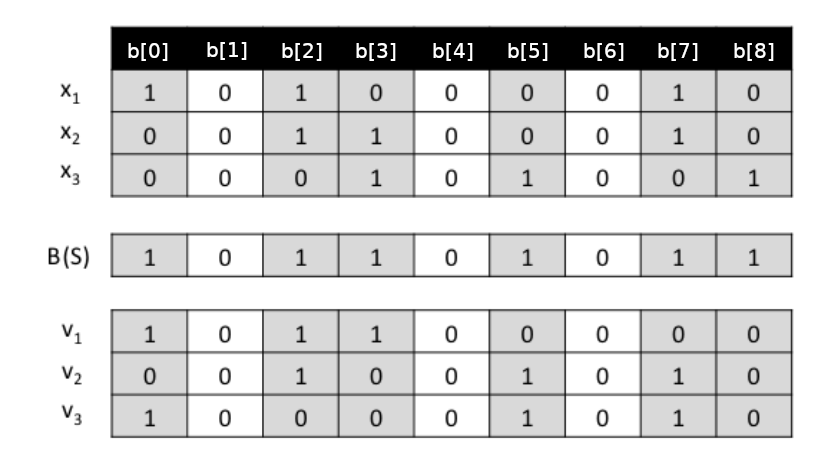
\includegraphics[width=0.8\linewidth]{image/gamma_deniability}
	\caption[مثالی از حاشاپذیری-$\gamma$]{
		یک فیلتر بلوم تشکیل شده از عناصر $\{x_1, x_2, x_3\}$ که سه عنصر $\{v_1, v_2, v_3\}$ را به عنوان خطای نوع دو می‌پذیرد\cite{Bianchi2012}.
		
	}
	\label{fig:gamma_deniability}
\end{figure}

در \cite{Kanemura2017} پیشنهاد داده است که فیلتر بلوم استفاده شده در پروتکل بیت‌کوین با توجه به معیار حاشاپذیری-$\gamma$  
\cite{Bianchi2012}،
ساخته شود. زیرا نرخ خطای نوع دو ($P_t$) به تنهایی برای سنجش حریم خصوصی فیلتر بلوم ساخته شده کافی نیست. به این ترتیب لازم است که طبق معادله \eqref{eq:gamma-deniability} در هر لحظه باتوجه به تعداد آدرس‌های یکتایی که از نقطه بررسی تا آخرین بلوک استخراج شده در زنجیره بلوکی نمایان شده‌اند ($N_u$) و $\gamma$، مقدار $P_t$ تعیین گردد. از آن‌جایی که محاسبه $N_u$ برای گره سبک غیرممکن است، در \cite{Kanemura2017} پیشنهاد شده است که از تکنیک رگرسیون خطی برای تخمین  $N_u$  استفاده شود. ضرایب مدل رگرسیون خطی، باید متناوبا (مثلا به صورت هفتگی) محاسبه گردد. این محاسبه می‌تواند به توسعه دهندگان نرم‌افزار که طرح ارائه شده در \cite{Kanemura2017}  را پیاده‌سازی می‌کنند، سپرده شود. به این ترتیب گره سبک می‌تواند مقدار $P_t$ را به نحوی تعیین کند که از امنیت فیلتر بلوم مطمئن گردد.

روش ارائه شده در \cite{Kanemura2017} دارای اشکالاتی است. یکی از اصلی‌ترین این اشکالات به روزرسانی متناوب فیلتر بلوم باتوجه به تخمین حاصل از $N_u$  است. طبق مقاله \cite{Gervais2014}، اگر گره کامل متخاصم به دو فیتلر بلوم که مربوط به یک گره سبک هستند دست پیدا کند، می‌تواند با دقت بیش‌تری آدرس‌های مربوط به گره سبک را حدس بزند. از این رو تولید متناوب فیلتر بلوم می‌تواند حریم خصوصی کاربر سبک را به خطر بیاندازد.
از ایرادات دیگر این روش می‌توان به افزایش $P_t$ در نتیجه به کار گیری از این طرح اشاره نمود. به این ترتیب، پهنای باند مورد نیاز زیادتر می‌شود. 

\subsection{فیلترکردن بلوک سمت کاربرسبک}
\label{BIP157}
در \cite{Osuntokun2017} پیشنهاد شده است که بر خلاف آن‌که گره سبک فیلتر بلوم را تولید کند و برای گره کامل ارسال نماید، گره کامل یک فیلتر از روی تمام دادگان یک بلوک ایجاد می‌کند. گره سبک به ازای هر بلوک جدید، فیلتر مربوطه را از گره کامل دریافت کرده و خودش بررسی می‌کند که آیا داده مورد نظرش در آن قرار دارد یا نه. اگر داده مورد نظر گره سبک در آن فیلتر قرار داشت، تمام بلوک را از گره کامل دریافت می‌کند.

\subsection{بازیابی اطلاعات خصوصی}
\label{PIR}
در مقاله \cite{Qin2019} از روش بازیابی اطلاعات خصوصی (PIR) جهت دریافت اطلاعات تراکنش‌ها از گره‌ کامل استفاده کرده است. بازیابی اطلاعات خصوصی به کاربران این امکان را می‌دهد که از یک پایگاه داده یا مجموعه‌ای از آن‌ها یک پرسمان انجام دهند، به گونه‌ای که سرور پایگاه داده نتواند اطلاعاتی راجع‌به کاربران درخواست دهنده و درخواست آن‌ها کسب نماید. در مقاله \cite{Qin2019}  از ترکیبی از دو رده بازیابی اطلاعات خصوصی، یعنی بازیابی اطلاعات خصوصی نظریه اطلاعاتی (IT-PIR) و محاسباتی (C-PIR) استفاده کرده است. این ترکیب در مقاله \cite{Devet2014} معرفی شده است. در ،C-PIR پرسمان توسط کاربر به نحوی کدگذاری می‌شود که پایگاه داده پاسخ مناسب را در اختیار کاربر قرار دهد اما چیزی از پرسمان و اطلاعات ذخیره شده متوجه نشود. تضمین این حریم خصوصی بر مبنای این فرض است که با اختیار داشتن توان پردازشی محدود، حل برخی مسئله‌ها  غیر ممکن یا سخت خواهد بود \cite{Devet2014}.

رده IT-PIR وابسته به فرض سخت بودن حل الگوریتم‌های پایه رمز نگاری با منابع محاسباتی محدود نیست. پروتکل‌های رده IT-PIR از چند سرور به صورت همزمان استفاده می‌کند. تا زمانی که سرورهایی که تبانی نمی‌کنند از یک تعدادی بیش‌تر باشد، حریم خصوصی کاربر تضمین می‌شود \cite{Devet2014}. 

یکی از نقص‌های IT-PIR آن است که در عمل راه حلی وجود ندارد که بتوان حداقل تعداد سرورهایی که تبانی نکنند را تامین کرد. به ویژه که یک سرور می‌تواند در شبکه حمله سیبیل\RTLfootnote{\lr{Sybil attack}}
را انجام دهد. از طرف دیگر یکی از نقص‌های اساسی C-PIR آن است که به خاطر آن‌که تنها وابسته به یک سرور است، امکان تشخیص پاسخ‌های ناقص یا غیر صحیح از طرف سرور پایگاه داده وجود ندارد \cite{Qin2019}. به بیان ساده‌تر، در کاربرد فعلی سروری که قرار است اطلاعات مربوط به زنجیره بلوکی را در اختیار کاربران سبک قرار دهد،‌ می‌تواند از انشعابی نامعتبر از زنجیره بلوکی استفاده نماید. چون گره سبک با گره‌های کامل دیگر ارتباط ندارد، نمی‌تواند متوجه این مشکل شود.

مقاله \cite{Qin2019} با استفاده از از روشی که در \cite{Devet2014} معرفی شده، از هر دوی  IT-PIR و  C-PIR استفاده کرده است. از این طریق به نقاط قوت هر دو روش دست پیدا کرده و تا حدی نقاط ضعف آن‌ها را برطرف کرده است. روش‌های بازیابی اطلاعات خصوصی عموما سرعت پایین و پیچیدگی محاسباتی بالا و همچنین مصرف پهنای باند بالایی دارند. در روش ارائه شده  \cite{Qin2019} برای رفع این مشکل، پایگاه‌های داده‌ در سه دسته هفتگی، ماهانه (احتمالا
$30$
روزه) و تمام-مدت نگهداری می‌شوند. از این طریق تاخیر و پهنای باند مصرفی برای گره‌های سبکی که نیاز به دریافت و ارزیابی تراکنش‌های جدید دارند، کاهش می‌یابد. در این روش به ازای اضافه شدن هر بلوک جدید به زنجیره بلوکی، اطلاعات بلوک جدید به دسته هفتگی اضافه می‌شود. بعد از پایان یک هفته (اضافه شدن $1008$ بلوک)، دسته هفتگی خالی شده و تمام اطلاعات آن به دسته ماهانه اضافه می‌شود. بعد از آنکه دسته ماهانه تکمیل شد (اضافه شدن $4320$ بلوک برای $30$ روز) اطلاعات آن به دسته تمام-مدت اضافه می‌شود. 


روش ارائه شده در \cite{Qin2019} مشکلاتی به همراه دارد، اول از همه آن‌که این روش نسبت به روش فیلتر بلوم \cite{Hearn2013} به صورت قابل ملاحظه‌ای پهنای باند بیشتری مصرف می‌کند. به عنوان مثال برای آنکه یک کاربر بخواهد اطلاعات یک تراکنش را که در دسته تمام-مدت قرار دارد، دریافت کند، لازم است $64.53$ مگابایت پهنای باند مصرف نماید؛ در حالی که در صورتی که از روش مرسوم فیلتر بلوم استفاده نماید، لازم است که $69.32$ کیلوبایت پهنای باند مصرف کند. البته لازم به ذکر است که هر چه تعداد تراکنش‌های درخواستی افزایش پیدا کند و از دسته‌های جدیدتر پرسمان صورت گیرد، اختلاف پهنای باند مصرفی نسبت به روش فیلتر بلوم کمتر می‌شود. مثلا، برای دریافت $100$ تراکنش از دسته هفتگی، لازم است مجموعا $33$ مگابایت اطلاعات دریافت شود و در روش مرسوم فیلتر بلوم این مقدار برابر $10.09$ مگابایت است.

دوم، آن که برای انجام بازیابی اطلاعات خصوصی، سرور پایگاه داده برای هر جدول مربوط هر دسته یک فایل مانیفست ایجاد می‌کند. این فایل مانیفست شامل ابعاد پایگاه‌داده و موقعیت هر داده است. این فایل در اختیار کاربر قرار داده می‌شود. کاربر با توجه به این مانیفست می‌تواند پرسمان‌هایی ایجاد نماید به طوری که اطلاعاتی از او نزد سرور فاش نشود. با به‌روز شدن هر دسته، حتی با اضافه شدن هر اطلاعات جدیدی از زنجیره بلوکی به دسته هفتگی، نیاز است که فایل مانیفست مربوط به آن دسته به‌روز شود. به این ترتیب نیاز است که کاربر مانیفست جدید را دریافت کند. اندازه فایل مانیفست برای پرسمان از پایگاه داده‌ای که تنها شامل بایت‌ تراکنش‌ها باشد و پرسمان از طریق TXID تراکنش صورت بگیرد، به این صورت است: هفتگی: $72.45$ مگابایت، ماهانه: $218.68$ مگابایت و تمام-مدت $3.30$ گیگابایت. البته لازم به ذکر است که نویسندگان مقاله \cite{Qin2019} می‌خواهند بعدا ساز و کاری به روش ارائه شده اضافه نمایند که کاربر سبک بدون نیاز به بارگیری فایل مانیفست، برای آنکه اطلاعات مشخصی را استخراج نماید، بتواند بدون از بین رفتن محرمانگی درخواستش، اطلاعات مورد نیازش را از مانیفست ذخیره شده در گره کامل دریافت نماید.

ایراد سوم این روش آن است که روشن است پرسمان از دسته تمام-مدت همچنان زمان‌بر است. از این رو در این مقاله پیشنهاد شده است که دسته تمام مدت به زیر دسته‌‌هایی تقسیم شود.  پرسمان کاربر سبک از زیر دسته‌های کوچک‌تر می‌تواند برای گره کامل متخاصم حاوی اطلاعاتی باشد. مثلا با تحلیل زیردسته‌هایی که از آن‌ها پرسمان انجام شده است، و همچنین کشف ارتباط بین آدرس‌ها با توجه به تراکنش‌های بیت‌کوین، به بخشی از آدرس‌های مربوط به یک کاربر سبک پی برد. علاوه بر این می‌توان به این نکته اشاره کرد که آدرس‌های یک زیر دسته قاعدتا همگی نرخ استفاده یکسانی ندارند. می‌توان فرض کرد که آدرس‌های پراستفاده‌تر احتمال پرسمان بیش‌تری از طرف کاربر سبک مالک آن داشته باشند. از این رو احتمال پرسمان آدرس‌های یک زیر دسته برابر نیست و این اطلاعاتی جانبی برای حدس آدرس درخواست شده محسوب می‌شود \cite{Niu2015}. در \cite{Qin2019} اشاره شده است که اگر این زیردسته‌ها به اندازه کافی بزرگ باشند، مثلا به اندازه دسته ماهانه، کار را برای گره متخاصم برای یافتن الگویی در پرسمان‌های کاربر سبک سخت‌تر می‌کنند. از طرف دیگر خود تقسیم‌بندی زمانی نیز باعث می‌شود که گره کامل متخاصم بتواند با توجه به دسته‌های زمانی‌ای که کاربر از آن‌ها درخواست می‌دهد به اطلاعات جانبی از کاربر سبک دست پیدا کند. 


آخرین ضعفی که می‌توان برای این روش \cite{Qin2019} نام برد، آن است که در این روش زمانی که بلوک‌های ظرفیت هر دسته تکمیل شد، مثلا برای دسته هفتگی $1008$ بلوک، آن دسته خالی شده و مقادیر آن به دسته دیگر، مثلا ماهانه، منتقل می‌شود. این معماری می‌تواند مشکلاتی به همراه داشته باشد. مثلا، کاربرانی که تراکنش‌های مربوط به آن‌ها در بلوک‌های پایانی هفته در زنجیره بلوکی ثبت می‌شود، خیلی زود تراکنششان وارد دسته ماهانه می‌شود. در نتیجه لازم است برای دستیابی به اطلاعات تراکنش مربوط به خود، هر چند که مدت زمان زیادی از آن نگذشته است، از دسته ماهانه پرسمان انجام دهد و به تبع آن پهنای باند زیادی مصرف کنند. به همین ترتیب برای تراکنش‌هایی که در بلوک‌های پایانی یک ماه ثبت می‌شوند می‌توان این مشکل را متصور شد. از طرفی دیگر اگر معماری به نحوی تغییر پیدا کند که به عنوان مثال دسته هفتگی شامل $1008$ عدد از آخرین بلوک‌هایی باشد که استخراج شده‌اند و به ازای اضافه شدن هر بلوک جدید، قدیمی‌ترین بلوک این دسته را وارد دسته ماهانه شود، باعث می‌شود که بروز رسانی دسته‌های ماهانه و به همین ترتیب دسته تمام-مدت هر $10$ دقیقه انجام شود که نه تنها سربار پردازشی بسیار زیادی برای گره کامل به وجود خواهد آورد، بلکه همه فایل‌های مانیفستی که مربوط به سه دسته هستند و نزد کاربر سبک است پس از ده دقیقه منقضی می‌شوند که با توجه به اندازه‌ٔ آن‌ها، به روزرسانی مداوم آن‌ها مرقون به صرفه نخواهد بود.

\subsection{محیط اجرای قابل اعتماد}
\label{SGX}

روش BITE
\cite{Matetic2019}
، از یک محیط اجرای قابل اعتماد (مانند 
SGX\RTLfootnote{\lr{Software Guard Extensions}}
\cite{SGX})
برای حفظ حریم خصوصی کاربران سبک بهره‌گیری می‌کند. 
محیط اجرای قابل اعتماد SGX در گره‌های کامل قرار گرفته و وظیفه پاسخ دهی به درخواستِ تایید تراکنش از طرف کاربر سبک را دارد. SGX از نرم‌افزارهایی که در خارج از آن اجرا می‌شوند (حتی سیستم‌عامل) مجزا و منزوی است و می‌تواند یکپارچگی و محرمانگی داده‌ها را در مقابل گره کامل متخاصم دارنده آن حفظ نماید. در نتیجه قادر است در حفظ حریم خصوصی کاربران سبک و صحت (یک‌پارچگی) پاسخ‌ به آن‌‌ها مفید باشد. به طوری که نه تنها باعث جلوگیری از فاش شدن اطلاعات گره سبک در برابر گره کامل دارنده آن می‌گردد بلکه می‌تواند گره سبک را مطمئن کند که اطلاعات دریافتی صحیح و کامل هستند. با این حال گره کامل می‌تواند با بررسی الگوی دسترسی SGX به یک حافظه خارجی،‌ مانند پایگاه‌ دادهٔ‌ تراکنش‌ها، آدرس کاربر درخواست دهنده را حدس بزند. همچنین SGX نسبت به حملات کانال جانبی متعددی آسیب‌پذیر است. در مقاله \cite{Matetic2019} سعی شده است با بهره‌گیری از روش بازیابی اطلاعات خصوصی و تکنیک‌های حفاظت از کانال جانبی، امنیت روش پیشنهاد شده را افزایش دهد.

مقاله \cite{Matetic2019} دو نوع راه حل ارائه داده‌ است. راه حل اول پنجره پویش (\lr{Scanning Window}) و راه حل دوم پایگاه داده ناآگاهانه (\lr{Oblivious Database}) نام دارد. در هر دو روش، تصدیق از راه دور صورت می‌گیرید و یک ارتباط امن در لایه انتقال(
TLS\RTLfootnote{\lr{Transport Layer Security}})
مابین کاربر سبک و SGX برقرار می‌شود. کاربر سبک آدرس مورد نظرش را برای SGX می‌فرستد و SGX با توجه به زنجیره بلوکی تمام اطلاعات مورد نیاز جهت درستی سنجی وجود تراکنش در زنجیره بلوکی را بدست آورده و برای کاربر سبک درخواست دهنده می‌فرستد. 

در روش پنجره پویش، برای نرمالایز کردن رابطه بین اندازه پاسخ‌ و اطلاعاتی که در واقع به آن‌ها دسترسی صورت گرفته است از یک روش پویش خاص استفاده می‌شود. همان‌طور که گفته شد گره کامل متخاصم می‌تواند با بررسی الگو دسترسی SGX به حافظه، آدرس(های) درخواست داده شده را حدس بزند، در این روش قرار است از حفظ حریم خصوصی کاربر سبک از طریق پنهان‌سازی الگو‌های دسترسی به داده‌ یا بلوک اطمینان حاصل شود. هدف اصلی این روش پنهان‌سازی کامل نسبت اندازه پاسخ (نشان‌دهنده تعداد تراکنش‌های بازگردانده شده به کاربر) و تعداد بلوک‌های پویش شده است. زیرا گره کامل متخاصم می‌تواند با مقایسه اندازه پاسخ تولید شده توسط گره کامل و همچنین تعداد بلوک‌های پویش شده توسط آن به بسامد تراکنش‌هایی که مربوط به آن آدرس هستند دست پیدا کند؛ در نتجیه آدرس مورد نظر گره سبک درخواست دهنده را حدس بزند.

در شکل \ref{fig:scanningwindow} جزئیات روش پنجره پویش را، که در آن نسبت اندازه پاسخ و تعداد بلوک‌های پویش شده ثابت می‌ماند، نشان داده می‌شود. در این روش بعضا بلوک‌های بیشتری پویش می‌شوند تا نسبت اندازه پاسخ با بلوک‌های پویش شده ثابت بماند. گره کامل متخاصم تنها می‌تواند بلوک‌هایی که به آن‌ها دسترسی صورت گرفته است را شناسایی کند و چیزی درمورد آدرسی که از طرف کاربر سبک ارسال شده است و یا تراکنش‌های بازگردانده شده نمی‌داند. در این روش برای آن‌که جلوی  حمله زمانی به الگوریتم گرفته شود، می‌توان اثبات مرکل را برای تمام تراکنش‌های موجود در بلوک‌های پویش شده محاسبه کرده و به محاسبهٔ اثبات مرکل، تنها برای تراکنش‌های مورد نظر کاربر درخواست دهنده، بسنده نکرد. به این ترتیب این روش بار پردازشی بسیار زیادی را متحمل خواهد شد. از طرف دیگر اگر که گره کامل متخاصم بتواند حملات کانال جانبی دیجیتال دانه‌بندی زیاد\RTLfootnote{\lr{High-granularity digital side-channel attacks}} را اجرا نماید به طوری که بتواند مسیر اجرای برنامه را با دانه‌بندی سطح دستورات مشاهده کند، می‌تواند تراکنش‌هایی که انتخاب شده‌اند را تشخیص دهد. در این مقاله، برای مقابله با این حملات از روشی مبتنی بر \cite{Rane2015} بهره می‌گیرد که بار پردازشی الگوریتم را افزایش می‌دهد.

\begin{figure}[h]
	\centering
	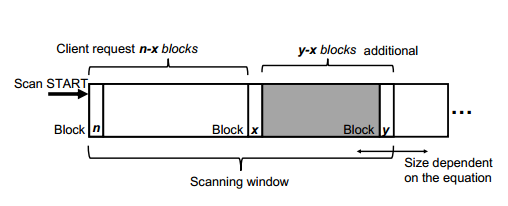
\includegraphics[width=0.7\linewidth]{image/Scanning_Window}
	\caption[پنجره پویش (\lr{Scanning Window}) ]{پنجره پویش. مطابق با تعداد بلوک‌های درخواست داده شده ($x$) و تعداد تراکنش‌های منطبق شده با درخواست مشتری در آن‌ها، احتمالا بلوک‌های بیشتری ($y$) از حافظه خوانده می‌شود تا نسبت بین بلوک‌های خوانده شده و اندازه پاسخ ثابت بماند\cite{Matetic2019}.}
	\label{fig:scanningwindow}
\end{figure}

روش دوم ارائه شده در \cite{Matetic2019} پایگاه داده ناآگاهانه نام دارد. در این روش کاربر سبک آدرس‌های مورد نظر خودش را، از طریق یک کانال محرمانه، برای SGX ارسال می‌کند و مستقیما اطلاعات مربوط به خروجی‌های خرج نشده را دریافت می‌نماید. در این روش برخلاف روش‌های پیشین و همچنین روش پنجره پویش،‌ نیاز نیست که کاربر سبک سرایند بلوک‌ها و مسیر (اثبات) درخت مرکل را دریافت و بررسی کند. در این روش کاربر به صحت عملکرد SGX و پاسخ آن اعتماد کامل دارد.
برای آنکه SGX بتواند کاربر را از صحت عملکرد خودش مطمئن سازد، 
تمام اقدامات و مقداردهی‌های اولیه به عنوان حالت اولیه ثبت می‌شود. با استفاده از آن کاربر می‌تواند مطمئن شود که کد صحیحی بر روی سامانه در حال اجرا است. به این فرایند تصدیق از راه دور\RTLfootnote{\lr{Remote Attestation}}
گفته می‌شود. تصدیق ایجاد شده، که شامل حالت اولیه است، امضا شده و برای کاربر ارسال می‌شود. کاربر می‌تواند توسط سرویس تصدیق برخطی که توسط اینتل ارائه می‌شود \cite{EPID}، امضا را بررسی نماید.

در روش پایگاه داده ناآگاهانه، SGX اطلاعات مربوط به خروجی خرج نشدهٔ تراکنش‌ها (UTXO) را در یک پایگاه داده رمزنگاری شده نگهداری می‌کند. همچنین از ماشین دسترسی تصادفی ناآگاهانهٔ
( ORAM\RTLfootnote{\lr{Oblivious Random Access Machine}})
معرفی شده در \cite{Stefanov2013} برای جلوگیری از نشت اطلاعات در هنگام دسترسی به حافظه استفاده می‌کند. به این ترتیب گره کامل متخاصم نمی‌تواند الگویی از دسترسی SGX به حافظه پیدا نماید. از طرف دیگر در این روش طول درخواست‌ها و پاسخ‌ها همواره یک مقدار ثابت است. اگر اندازه آن‌ها از آن مقدار ثابت کوتاه‌تر باشد، با لایی‌گذاری و اگر طولانی‌تر بود با تکه‌تکه کردن، به اندازه‌های ثابت تبدیل می‌شوند. در این روش SGX به تمام زنجیره بلوکی دسترسی ندارد و تنها دادهٔ UTXO را نگهداری کرده و به ازای اضافه شدن هر بلوک جدید، بعد از آن که آن بلوک را از جنبه اثبات کار و درخت مرکل درستی سنجی کرد، آن را به روزرسانی می‌کند. از آن‌جایی که UTXO در حافظه ORAM ذخیره می‌گردد، به روزرسانی آن امری نسبتا زمان‌بر، چیزی در حدود $78.5$ ثانیه، خواهد بود.

در دو روش ارائه شده در \cite{Matetic2019} بار پردازشی چندانی بر روی گره سبک قرار نخواهد گرفت. همچنین از آن‌جایی که دیگر لازم نیست برای حفظ حریم خصوصی کاربر تراکنش‌هایی مازاد به خاطر خطای نوع دو نیز دریافت شوند، پهنای باند به طور قابل ملاحظه‌ای در این دو روش نسبت به روش فیلتر بلوم کاهش پیدا می‌کند. از طرف دیگر در روش دوم (پایگاه داده ناآگاهانه) نیاز نیست که پاسخ گره کامل با اثبات‌های مرکل همراه باشد و به عبارتی گره سبک به عملکرد صحیح SGX اعتماد دارد. در نتیجه در این روش پهنای باند مصرفی بسیار کاهش پیدا می‌کند. علاوه بر مزایای ذکر شده، این روش ایراداتی نیز دارد که در ادامه به بیان آن خواهیم پرداخت.

اول از همه آنکه زمان تولید جواب در روش پنجره پویش، در صورتی که اقدامت مورد نیاز جهت جبران حمله کانال جانبی انجام شود، بسیار زمان‌بر است. به عنوان مثال برای پردازش  $100$ بلوک در این روش چیزی در حدود $73$ ثانیه زمان نیاز است. این زمان برای روش فیلتر بلوم با نرخ خطای نوع دوی $0.5$ درصد، حدود $1.1$ ثانیه است \cite{Matetic2019}. هر چند که تولید پاسخ در روش  پایگاه داده ناآگاهانه بسیار سریع‌تر انجام می‌شود، اما برای به روز رسانی داده خروجی‌ خرج نشده تراکنش‌ها نیاز به $78.5$ ثانیه زمان دارد. به عبارتی می‌توان اینطور گفت که هر ده دقیقه یک‌بار (زمان مورد نیاز برای استخراج یک بلوک جدید)، حدود یک دقیقه و هجده ثانیه،‌ صرف به روز رسانی شده و امکان پاسخ‌گویی به کاربران سبک را ندارد. مقاله \cite{Matetic2019} برای افزایش دسترس‌پذیری سیستم در شرایط به روز رسانی، پیشنهاد استفاده از دو سیستم موازی را داده است. در این شرایط نیز،‌ سیستم ارائه دهنده خدمات از وضعیت فعلی شبکه حداکثر حدود $78.5$ ثانیه عقب‌تر خواهد بود.

مشکل دیگری که روش \cite{Matetic2019} دارد، حملات فیزیکی مدرنی است که SGX نسبت به آن‌ها آسیب‌پذیر است. مثلا حملات اسپکتر\RTLfootnote{\lr{Spectre}}\cite{Kocher2019}، ملت‌داون\RTLfootnote{\lr{Meltdown}}\cite{Lipp2020} و حمله \cite{Bulck2020} که به تازگی کشف شده است، می‌توانند برای استخراج کلید‌های تصدیق از ‌SGX مورد استفاده قرار گیرند. در صورتی که گره کامل متخاصم از چنین حمله‌ای بهره‌بردای کند، می‌تواند در روش پنجره پویش، حریم خصوصی کاربران سبک درخواست دهنده را نقض نماید؛ همچنین در روش پایگاه دادهٔ ناآگاهانه علاوه بر نقض حریم خصوصی کاربر سبک می‌تواند اطلاعات اشتباهی را در اختیار وی قرار دهد.

علاوه بر مشکلات ذکر شده در بالا، می‌توان به این مسئله نیز اشاره نمود که برای آنکه یک گره کامل بخواهد خدمات پیشنهاد شده در \cite{Matetic2019} را به گره‌های سبک ارائه دهد، نه تنها نیاز است که یک محیط اجرای قابل اطمینان تهیه و راه‌اندازی نماید، بلکه لازم است که منابع پردازشی قابل توجهی را برای این منظور اختصاص دهد. در نتیجه گره‌های کاملی که بتوانند چنین خدماتی ارائه دهند، محدود خواهند بود. به تبع آن کاربران سبک مجبور خواهند بود که بین گره‌های کامل محدود‌تری انتخاب کنند که این مسئله انگیزه این گره‌های کامل را برای انجام اقدامات خصمانه بیشتر خواهد کرد. از این اقدامات می‌توان به ایجاد و دنبال کردن یک انشعاب ناصحیح از زنجیره بلوکی بیت‌کوین اشاره نمود. در حالت عادی که تعداد گره‌های کامل زیاد هستند، گره سبک می‌تواند با دریافت خدمات از گره‌های کامل متعدد از صحت اطلاعات دریافتی مطمئن گردد.

از طرف دیگر، شرکت‌های محدودی مانند اینتل، تجهیزات مربوط به یک محیط اجرای قابل اطمینان را تولید و به فروش می‌رسانند. همچنین نیاز است که برای  تصدیق از راه دور عملکرد آن‌ها به سرویس‌هایی مثل \cite{EPID} وابسته بود. به بیان دیگر می‌توان این طور گفت که برای آنکه بتوان از روش \cite{Matetic2019} بهره‌برداری کرد، لازم است به شرکت‌های محدودی اعتماد شود که این خود بر خلاف ذات شبکه‌های همتابه‌همتایی مثل بیت کوین است.



\section{نتیجه‌گیری}
‌در نتیجه‌گیری آخر این فصل، با توجه به بررسی انجام شده بر روی مراجع تحقیق، بخش‌های قابل گسترش و تحقیق در آن حیطه و چشم‌اندازهای تحقیق مورد بررسی قرار می‌گیرند.	در برخی از تحقیقات، نتیجه نهایی فصل روش تحقیق، ارائهٔ یک چارچوب کار تحقیقی 
\lr{(research framework)}
است.